\section{Generalizing the \il{put} and \il{get} operations}\label{s:lvars-generalizing}

The determinism result for $\lambdaLVar$ shows that adding a store of
LVars, and the accompanying interface of @new@/@put@/@get@ operations,
to an existing deterministic parallel language (the
$\lambda$-calculus) preserves determinism.  But it is not the case
that the @put@ and @get@ operations are \emph{the most general}
interface that preserves determinism.  In this section, I consider
some alternative semantics for @put@ and @get@ that generalize their
behavior while retaining the determinism of the original semantics.

\subsection{Generalizing from least-upper-bound writes to inflationary, commutative writes} 

\lk{This will be about generalized inflationary+commutative writes,
  rather than least-upper-bound writes (lub is a special case of
  this).}

\TODO{Say something about how the lattice in
  Figure~\ref{f:lvars-example-lattices}(c) has different semantics if
  we have least-upper-bound writes or incremental writes, and how
  incremental writes may in fact be what is desired.  Possibly cite
  the CRDTs work and forward-reference Chapter~\ref{ch:distributed}.}

\lk{Following stuff is from the WoDet paper.}

As we have seen, CvRDTs support inflationary updates---that is,
updates that are nondecreasing with respect to the lattice in
question---that are not necessarily join operations.  Indeed, the
\emph{only} requirement on a CvRDT update is that it be inflationary.
With LVars, on the other hand, all updates are joins.  In this section
we propose adding inflationary non-join updates to the LVars model.

As a canonical example of an LVar update that cannot be directly
modeled as a join, consider an atomically incremented counter that
occupies one memory location.  Atomic increments to such a counter are
efficient, commutative, and ultimately fit well inside the LVar
framework.  Atomic increment is a useful primitive---an example use
case is
\emph{PhyBin}\footnote{\url{http://hackage.haskell.org/package/phybin}},
a bioinformatics application that we parallelized with
LVish~\cite{effectzoo}.  PhyBin uses atomic increment operations to
gradually build a distance matrix, concurrently incrementing the
distance in each cell of the matrix.

More generally, for an LVar with lattice $(D,\leq,\bot, \top)$, a data
structure author may define a set of {\em bump} operations $\BUMP_i :
D \rightarrow D$, which must meet the following two conditions:
\begin{itemize}
\item $\forall a, i.     \;\; a \leq \BUMP_i(a) $
\item $\forall a, i, j.  \;\; \BUMP_i(\BUMP_j(a)) = \BUMP_j(\BUMP_i(a)) $
\end{itemize}
When extending LVish to include @bump@, we must keep in mind that
@bump@ and @put@ operations on the same LVar do not necessarily mix.
For example, consider a set of @bump@ operations $\{\BUMP_{(+1)},
\BUMP_{(+2)}, \dots \}$ for atomically incrementing a counter
represented by a natural number LVar, with a lattice ordered by the
usual $\leq$ on natural numbers.  A @put@ of $4$ and a $\BUMP_{(+1)}$
do not commute!  If we start with an initial state of $0$ and the
@put@ occurs first, then the state of the LVar changes to $4$ since
$\max(0, 4) = 4$, and the subsequent $\BUMP_{(+1)}$ updates it to $5$.
But if the $\BUMP_{(+1)}$ happens first, then the final state of the
LVar will be $\max(1, 4) = 4$.  Furthermore, multiple distinct
families of @bump@ functions only commute among themselves and cannot
be combined.  In fact, @put@ operations themselves, with their
underlying join operations on the single state replica, meet the above
two conditions for @bump@, and therefore can be viewed as a special
case of @bump@ that, in addition to being inflationary, also happens
to compute a join.

Fortunately, in the LVish library, the author of a particular LVar
data structure can choose what operations that data structure should
provide, and the Haskell type system will statically rule out programs
that attempt to use other, incompatible @bump@ operations on the same
LVar.  Moreover, it is safe to \emph{compose} LVars that support
different families of @bump@ operations.  For example, if we defined a
@Counter@ LVar type with a @bump@ operation, an LVar of type \il{Set
  Counter} could contain a monotonically growing set of @bump@-able
counters that each monotonically increase.  What remains is to
formally define the operational semantics of @bump@ and update the
determinism proofs for LVar calculi~\cite{LVars-paper, Freeze-paper}
to account for it; we expect this to be a straightforward change to
the existing proofs.

\lk{Following stuff is from the PLDI paper.}

In the original LVars model~\cite{LVars-paper,Freeze-paper}, the only
way for the state of an LVar to evolve over time is through a series
of least-upper-bound (lub) updates resulting from calls to @put@
operations.

Unfortunately, this way of updating an LVar provides no efficient way
to model an atomically incremented counter that occupies one memory
location.  Yet, atomic increments to such a counter are efficient,
commutative, and ultimately fit well inside the LVish framework.
Hence the most basic extension we make to LVish is to (optionally)
relax its reliance on idempotence of operations.  Thereafter we can
safely add a restricted set of atomic read-modify-write operations
that are inflationary with respect to a lattice, but do not compute a
lub.  \lk{we introduce the term ``inflationary'' earlier, don't need
  to italicize it here} We will see one example of an application that
critically requires this functionality in Section~\ref{s:phybin}.

We consider a new family of LVar update operations that are required
to commute and be inflationary with respect to the lattice in
question, but are not limited to the lub semantics of @put@.
Specifically, for a lattice $(D,\userleq,\bot, \top)$, a data
structure author may define a set of {\em bump} operations $\BUMP_i :
D \rightarrow D$, which must meet the following two conditions:
\begin{itemize}
\item $\forall a, i.     \;\; a \userleq \BUMP_i(a) $
\item $\forall a, i, j.  \;\; \BUMP_i(\BUMP_j(a)) = \BUMP_j(\BUMP_i(a)) $
\end{itemize}
As a simple example, consider an LVar whose states are natural
numbers, with $0$ as the least element and with the usual $\leq$
operation on natural numbers as the ordering on states.  The ordering
induces a lub operation equivalent to the $\max$ operation on natural
numbers.  We can implement a family of @bump@ operations that
increment the LVar by various amounts: $\{ (+1), (+2), (+3), \dots
\}$.

A critical point to note, however, is that it is not safe to update
the same LVar with {\em both} @put@ and @bump@.  For example, a @put@
of $4$ and a $\BUMP_{(+1)}$ do not commute!  If we start with an
initial state of $0$ and the @put@ occurs first, then the state of the
LVar changes to $4$ since $\max(0, 4) = 4$, and the subsequent
$\BUMP_{(+1)}$ updates it to $5$.  But if the $\BUMP_{(+1)}$ happens
first, then the final state of the LVar will be $\max(1, 4) = 4$.
{Furthermore, multiple distinct families of @bump@ functions only
  commute among themselves and cannot be combined.}  In practice, this
distinction is enforced by the type system. For example, the
LVish-provided set data structure @Data.LVar.Set@ supports only @put@,
whereas @Data.LVar.Counter@ supports only @bump@.

{\em Composing} these data structures, however, is fine.  For example,
an LVar could represent a monotonically growing collection (which
supports @put@) of counter LVars, where each counter is itself
monotonically increasing and supports only @bump@.  Indeed, the PhyBin
application described in Section~\ref{s:phybin} uses just such a
collection of counters.

\paragraph{Determinism guarantee}

The determinism of LVish \cite{LVars-paper} relies on the fact that
the states of all LVars evolve monotonically with respect to their
lattices, and that the lub operation is commutative and therefore the
order in which @put@s occur does not matter.  Together, these
properties suffice to ensure that the threshold reads made by @get@
operations are deterministic. The rest of an LVish program is purely
functional, and its behavior is, in fact, a pure function of these
@get@ observations.  Since @bump@ operations are also commutative and
inflationary with respect to the lattice of the LVar they operate on,
we see that they preserve determinism, as long as programs do not use
@bump@ and @put@ on the same LVar.  \lk{I don't want to cite the CRDT
  proof here.  They say that state-based CRDTs (put) can be simulated
  with op-based CRDTs (bump) and vice versa.  But they do \emph{not}
  say that lattice monotonicity is preserved.  With op-based CRDTs
  there is no notion of a lattice to be preserved.}

We can go further and generalize this argument, and in fact will need
to for the other extensions described in this paper.  Consider LVish
with @put@, @bump@, and @get@ effects.  By commutativity, we can
reduce the effects in a program execution to three {unordered sets}:
$(P,B,G)$.  By slicing the system at this interface, we can decompose
determinism proof obligations into two parts:
\label{s:multiagent}
\begin{itemize}
\item The LVish (Haskell) code must guarantee that it implements a
  monotone function $\mathcal P(G) \rightarrow \mathcal P(P) \times
  \mathcal P(B)$.  That is, adding more @get@ results on the left
  results only in {\em more} @put@/@bump@ effects on the right (as
  more @get@s unblock and run, more @put@ and @bump@ operations can
  run); furthermore, those effects are a function of nothing {\em
    other} than @get@.
\item The mutable (but monotonically growing) heap of LVars must
  likewise guarantee that the set of @get@ results is a pure function
  of the set of @put@s and @bump@s.  This is straightforward to show,
  given the lattice-based semantics of @put@ and @bump@.
\end{itemize}
This {\em communicating agents} formulation of determinism for LVish
puts us in a position to replace the monotonically growing heap with
other deterministic agents that fulfill the same contract, as we will
see in Section~\ref{s:parST}.
%
At that point, we will also discuss \emph{temporal contracts} on the order of
operations, going beyond the simple case of completely unordered sets at the
interfaces.
\lk{Not gonna lie---I find this part about ``communicating agents''
  fuzzy and unconvincing.}

\paragraph{Deleveraging idempotency}\label{s:dedup}

Since lub is an idempotent operation, the previously existing LVish
implementation assumed idempotence of all writes, which in turn
enabled the scheduler to relax synchronization requirements at the
cost of low-probability duplication of
work~\cite{Freeze-paper}. Adding support for operations like @bump@
makes this assumption untenable.  Therefore, we re-engineered the
LVish runtime system to (optionally) include additional
synchronization.\footnote{Space constraints preclude full description
  here, but the key challenge is resolving a race between \il{put}s
  and attempts to register new handlers (callbacks) on an LVar.  Our
  solution is a specialized variant of a reader-writer lock that
  requires zero writes to shared addresses if no handlers are
  currently being registered.}

\paragraph{Fine-grained effect tracking}

\lk{How's this?  It avoids having to explain freeze.}
Naturally, it is best to pay the aforementioned synchronization
overhead only when required.  This requires static information about
whether a given program uses @bump@.  With that as one of our goals, 
we extend LVish
to allow for \emph{static fine-grained effect tracking}.  The idea is
to guarantee that only certain LVar effects can occur within a given
@Par@ computation.  In Haskell, we can do so at the type level
by indexing @Par@ computations with a \emph{phantom type} @e@ that
indicates their \emph{effect level}.  That is, the @Par@ type
 becomes, instead, @Par e@, where @e@ 
is a type-level encoding of booleans indicating whether or not writes,
reads, non-idempotent (@bump@), or non-deterministic (@IO@) operations
are allowed to run inside it.

Moreover, in real LVish programs, the @Par@ type constructor has a
second type parameter, @s@, making @Par e s a@ the complete type of a
computation that returns a result of type @a@.\footnote{To be precise,
  in the earlier 1.x releases of LVish, the \il{e} type parameter for
  effect level was instead \il{d}, for ``determinism level'', and was
  a simple type-level boolean switch distinguishing deterministic from
  {\em quasi-deterministic} \il{Par} computations~\cite{Freeze-paper}.
  The effect signatures in this paper generalize determinism levels
  and correspond to the newer LVish 2.x API.}  The @s@ parameter
ensures that it is not possible to reuse an LVar from one @runPar@
session to the next, just as the @ST@ monad in Haskell prevents an
@STRef@ from escaping @runST@; likewise the types of individual LVars
must be parameterized by @s@ as well.  For simplicity of presentation,
we elided the @e@ and @s@ type parameters in
Section~\ref{s:refresher}, instead following the simpler @Par a@
format of the earlier \emph{monad-par} library~\cite{monad-par}, but
we include them from this point onward.

To enable future additions of effect ``switches'' \new{encoded in
  \il{e}}, we follow the precedent of recent work by Kiselyov \etal~on
extensible effects in Haskell~\cite{oleg-amr-haskell-2013}: we
abstract away the specific structure of @e@ into \emph{type class
  constraints}, which allow a @Par@ computation to be annotated with
the \emph{interface} that its @e@ type parameter is expected to
satisfy.  For example, a @Par@ computation annotated with the effect
level constraint @HasPut@ can perform @put@s.  Thus the signature for
the @put@ operation on IVars becomes:

\begin{lstlisting}
   put :: HasPut e => IVar s a -> a -> Par e s ()
\end{lstlisting}
while the signature for an @incrCounter@ operation uses the
@HasBump@ constraint:
\begin{lstlisting}
   incrCounter :: HasBump e => Counter s -> Par s e ()
\end{lstlisting}
These constraints can also be \emph{negative}.  For example, the
@runPar@ function for executing @Par@ computations in a purely
functional context requires the absence of explicit freeze or IO
operations:
\begin{lstlisting}[mathescape=true]
runPar :: (NoFreeze e, NoIO e) => (forall s $.$ Par e s a) ->  a 
\end{lstlisting}

\subsection{A more general formulation of threshold sets}\label{subsection:lvars-a-more-general-formulation-of-threshold-sets}

Certain deterministic computations are difficult to express using our
existing definition of threshold sets.  For instance, consider an LVar
that stores the result of a parallel logical ``and'' operation on two
Boolean inputs.  I'll call this data structure an \emph{\il{AndLV}},
and its two inputs the \emph{left} and \emph{right} inputs,
respectively.

We can represent the states an \il{AndLV} can take on as pairs
\il{(x,y)}, where each of \il{x} and \il{y} are \il{T}, \il{F}, or
\il{Bot}.  The \il{(Bot,Bot)} state is the state in which no input has
yet been received, and so it is the least element in the lattice of
states that our \il{AndLV} can take on, shown in
Figure~\ref{f:lvars-parallel-and}.  An additional state, \il{Top}, is
the greatest element of the lattice; it represents the situation in
which an error has occurred---if, for instance, one of the inputs
writes \il{T} and then later changes its mind to \il{F}.

\begin{figure}
\begin{center}
  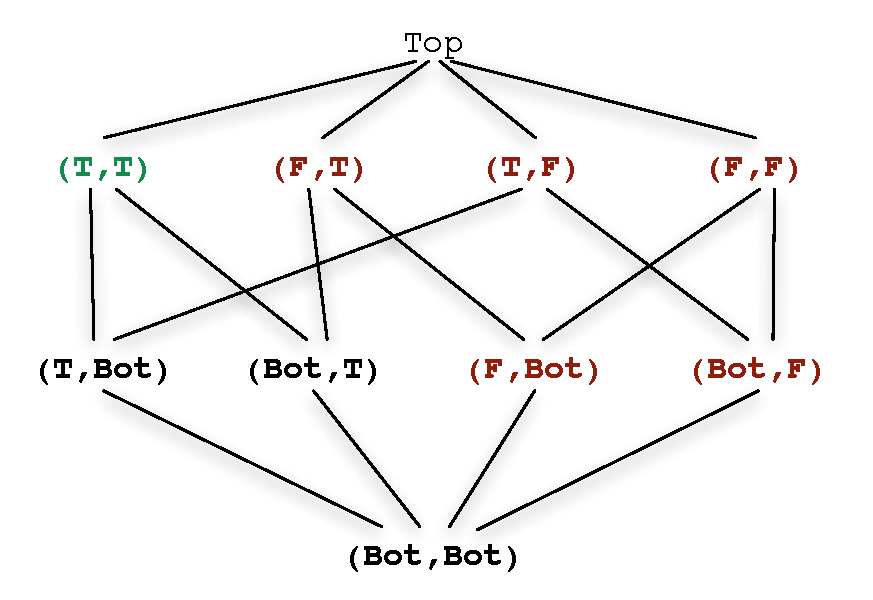
\includegraphics[width=3in]{chapter2/figures/lvars-parallel-and.pdf}
\end{center}
  \caption{Lattice of states that an \il{AndLV} can take on.  The five
    red states in the lattice correspond to a false result, and the
    one green state corresponds to a true one.}
  \label{f:lvars-parallel-and}
\end{figure}

The lattice induces a lub operation on pairs of states; for instance,
the lub of \il{(T,Bot)} and \il{(Bot,F)} is \il{(T,F)}, and the lub of
\il{(T,Bot)} and \il{(F,Bot)} is \il{Top} since the overlapping \il{T}
and \il{F} values conflict.  As usual for LVars, the @put@ operation
updates the \il{AndLV}'s state to the lub of the incoming state and
the current state.

We are interested in learning whether the result of our parallel
``and'' computation is ``true'' or ``false''.  Let's consider what
observations it is possible to make of an \il{AndLV} under our
existing definition of threshold reads.  The states \il{(T,T)},
\il{(T,F)}, \il{(F,T)}, and \il{(F,F)} are all pairwise incompatible
with one another, and so $\setof{\textrm{ \il{(T,T)}, \il{(T,F)},
    \il{(F,T)}, \il{(F,F)} }}$---that is, the set of states in which
both the left and right inputs have arrived---is a legal threshold set
argument to @get@.  The trouble with this threshold read is that it
does not allow us to get \emph{early answers} from the computation.
It would be preferable to have a @get@ operation that would ``short
circuit'' and unblock immediately if a single input of, say,
\il{(F,Bot)} or \il{(Bot,F)} was written, since no later write could
change the fact that the result of the whole computation would be
``false''.\footnote{Actually, this is not quite true: a write of
  \il{(F,Bot)} followed by a write of \il{(T,Bot)} would lead to a
  result of \il{Top}, and to the program stepping to the $\error$
  state, which is certainly different from a result of ``false''.
  But, even if a write of \il{(T,Bot)} is due to come along sooner or
  later to take the state of the \il{AndLV} to \il{Top} and thus raise
  $\error$, it should still be fine for the \il{get} operation to
  allow ``short-circuit'' unblocking, because the result of the
  \il{get} operation does not count as observable under our definition
  of observable determinism (as discussed in
  Section~\ref{subsection:lvars-errors-and-observable-determinism}).}
Unfortunately, we cannot include \il{(F,Bot)} or \il{(Bot,F)} in our
threshold set, because the resulting threshold set would no longer be
pairwise incompatible, and therefore would compromise determinism.

In order to get short-circuiting behavior from an \il{AndLV} without
compromising determinism, we need to make a slight generalization to
how threshold sets and threshold reads work.  In the new formulation,
we divide up threshold sets into subsets that we call \emph{activation
  sets}, each consisting of \emph{activation states}.  In the case of
the observation we want to make of our \il{AndLV}, one of those
activation sets is the set of states that the data structure might be
in when a state containing at least one \il{F} value has been
written---that is, the set $\setof{ \textrm{\il{(F,Bot)},
    \il{(Bot,F)}, \il{(F,T)}, \il{(T,F)}, \il{(F,F)}} }$.  When we
reach a point in the lattice that is at or above any of those states,
we know that the result will be ``false''.  The other activation set
is the singleton set $\{ \textrm{\il{(T,T)}} \}$, since we have to
wait until we reach the state \il{(T,T)} to know that the result is
``true''; a state like \il{(T,Bot)} does not appear in any of our
activation sets.

We can now redefine ``threshold set'' to mean \emph{a set of
  activation sets}.  Under this definition, the entire threshold set
that we would use to observe the contenst of our \il{AndLV} is:
\[
\{ 
\{ \textrm{\il{(F,Bot)}, \il{(Bot,F)}, \il{(F,T)}, \il{(T,F)}, \il{(F,F)}} \},
\{ \textrm{\il{(T,T)}} \}
\}
\]
We redefine the semantics of @get@ as follows: if an LVar's state
reaches (or surpasses) any state or states in a particular activation
set in the threshold set, @get@ returns \emph{that entire activation
  set}, regardless of which of its activation states was reached. If
no state in any activation set in the threshold set has yet been
reached, the @get@ operation will block.  In the case of our
\il{AndLV}, as soon as either input writes a state containing an
\il{F}, our @get@ will unblock and return the first activation set,
that is, $\{ \textrm{\il{(F,Bot)}, \il{(Bot,F)}, \il{(F,T)},
  \il{(T,F)}, \il{(F,F)}} \}$.  Hence \il{AndLV} has the expected
``short-circuit'' behavior and does not have to wait for a second
input if the first input contains an \il{F}.  If, on the other hand,
the inputs are \il{(T,Bot)} and \il{(Bot,T)}, the @get@ will unblock
and return $\{ \textrm{\il{(T,T)}} \}$.

In a real implementation, of course, the value returned from the @get@
could be more meaningful to the client---for instance, a Haskell
implementation could return \il{False} instead of returning the actual
activation set that corresponds to ``false''.  However, the
translation from $\{ \textrm{\il{(F,Bot)}, \il{(Bot,F)}, \il{(F,T)},
  \il{(T,F)}, \il{(F,F)}} \}$ to \il{False} could just as easily take
place on the client side.  In either case, the activation set returned
from the threshold read is the same regardless of \emph{which} of its
activation states caused the read to unblock, and it is impossible for
the client to tell whether the actual state of the lattice is, say,
\il{(T,F)}, \il{(F,F)}, or some other state containing \il{F}.

As part of this new formulation based on activation sets, we need to
adjust our criterion for pairwise incompatibility of threshold sets.
Recall that the purpose of the pairwise incompatibility requirement
(see Section~\ref{subsection:lvars-communication-primitives}) was to
ensure that a threshold read would return a unique result.  We need to
generalize this requirement, since although more than one element
\emph{in the same activation set} might be reached or surpassed by a
given write to an LVar, it is still the case that writes should only
unblock a \emph{unique} activation set in the threshold set.  The
pairwise incompatibility requirement then becomes that elements in an
activation set must be \emph{pairwise incompatible} with elements in
every other activation set.  That is, for all distinct activation sets
$Q$ and $R$ in a given threshold set:
%
\[ \forall q \in Q.~\forall r \in R.~q \sqcup r = \top \]
%
In our \il{AndLV} example, there are two distinct activation sets, so
if we let $Q = \{ \textrm{\il{(T,T)}} \}$ and $R = \{
\textrm{\il{(F,Bot)}, \il{(Bot,F)}, \il{(F,T)}, \il{(T,F)},
  \il{(F,F)}} \}$, the least upper bound of \il{(T,T)} and $r$ must be
\il{Top}, where $r$ is any element of $R$.  We can easily verify that
this is the case.  Furthermore, since the lattice of states that an
\il{AndLV} can take on is finite, the join function can be verified to
compute a least upper bound.

To illustrate why we need pairwise incompatibility to be defined this
way, consider the following (illegal) ``threshold set'' that does not
meet the pairwise incompatibility criterion:
\[
\{ 
\{ \textrm{\il{(F,Bot)}, \il{(Bot,F)}} \},
\{ \textrm{\il{(T,Bot)}, \il{(Bot,T)}} \}
\}
\]
A threshold read corresponding to this so-called threshold set will
unblock and return $\{ \textrm{\il{(F,Bot)}, \il{(Bot,F)}} \}$ as soon
as a state containing an \il{F} is reached, and $\{
\textrm{\il{(T,Bot)}, \il{(Bot,T)}} \}$ as soon as a state containing
a \il{T} is reached.  If, for instance, the left input writes
\il{(F,Bot)} and the right input writes \il{(Bot,T)}, and these writes
occur in arbitrary order, the threshold read will return a
nondeterministic result, depending on the order of the two writes.
But, with the properly pairwise-incompatible threshold set above, the
threshold read will block until the write of \il{(F,Bot)} arrives, and
then will deterministically return the ``false'' activation set,
regardless of whether the write of \il{(Bot,T)} has arrived yet.
Hence ``short-circuit'' evaluation is possible.

\lk{It'd be nice to have better terminology for these than just
  ``old-style threshold sets'' and ``new-style threshold sets''.}

Finally, we can mechanically translate old-style threshold sets into
new-style threshold sets and retain the old semantics.  In the
translation, every member of the old-style threshold set simply
becomes a singleton activation set. So, if we wanted a
non-short-circuiting threshold read under the new system, our
threshold set would simply be
\[
\{ 
\{ \textrm{\il{(T,T)}} \},
\{ \textrm{\il{(T,F)}} \},
\{ \textrm{\il{(F,T)}} \},
\{ \textrm{\il{(F,F)}} \}
\},
\]
which is legal under the new formulation.

\subsection{Generalizing from threshold sets to threshold functions}

\TODO{Write this subsection!}

\lk{This will be about "threshold functions", rather than either
  simple threshold sets or generalized threshold sets (i.e., partial
  functions that take a lattice element and are undefined for all
  inputs that are not at or above a given point in the lattice, and
  constant for all inputs that are at or above that point; both kinds
  of threshold sets are a special case of this, afaict).}
